\documentclass[10pt,twocolumn,letterpaper]{article}
\usepackage{microtype}
\usepackage{booktabs}
\usepackage{hyperref}
\usepackage{amsmath}
\usepackage{graphicx}
\usepackage{cleveref}

\title{MLOps Agéntico: Orquestación Autónoma de Clústeres de Entrenamiento de Visión Distribuida Impulsada por LLM usando Model Context Protocol (MCP)}
\author{William Steve Rodriguez Villamizar (wisrovi rodriguez)\\AI Leader \& Solutions Architect\\wisrovi-suit (https://github.com/wisrovi/w-cli)}
\date{}
\raggedbottom
\begin{document}
\maketitle

\section{Resumen \& Palabras Clave}
\textbf{Resumen:} Las arquitecturas tradicionales de Operaciones de Machine Learning (MLOps) enfrentan desafíos de escalabilidad y estabilidad al escalar cargas de trabajo de visión por computadora distribuidas. Presentamos un marco de investigación aplicada utilizando el Protocolo de Contexto de Modelo (MCP) para conectar Grandes Modelos de Lenguaje (LLMs) y clústeres físicos de GPU. Al aislar los nodos del clúster mediante un patrón Invocador-Ejecutor a través de demonios Celery, mitigamos efectivamente los fallos catastróficos de Fuera de Memoria (OOM) que frecuentemente bloquean los procesos host durante sesiones intensas de entrenamiento YOLO. Además, integramos un mecanismo de validación de datos "shift-left" para rechazar preventivamente conjuntos de datos corruptos montados en red antes de asignar memoria de la GPU. Las evaluaciones empíricas frente a líneas base de la industria (Ray Train y Kubernetes) demuestran que este enfoque redujo la latencia de orquestación, disminuyó el consumo pico de memoria de un inestable 28GB a un límite estricto de 16GB, y previno por completo las caídas por OOM durante una prueba de estrés de 72 horas. La integración de LLMs como gestores autónomos del clúster demuestra un ejemplo concreto de investigación aplicada que produce resultados robustos y reproducibles para la comunidad de ingeniería de ML.

\textbf{Palabras Clave:} MLOps Agéntico, Model Context Protocol, Computación Distribuida, Orquestación LLM, Validación Shift-Left.

\section{Información del Autor}
Esta investigación fue conceptualizada y desarrollada por William Steve Rodriguez Villamizar (wisrovi rodriguez), AI Leader \& Solutions Architect para el ecosistema wisrovi-suit (https://github.com/wisrovi/w-cli).

\section{Introducción}
Escalar clústeres de entrenamiento distribuido para modelos de visión por computadora de alta resolución presenta desafíos de ingeniería severos. Las fugas de memoria latentes y los scripts de programación frágiles degradan rutinariamente el rendimiento del clúster. Los investigadores encuentran frecuentemente caídas silenciosas por Fuera de Memoria (OOM) donde el demonio de entrenamiento principal asigna memoria más allá de los límites físicos de la GPU, bloqueando todo el nodo y requiriendo reinicios forzados manuales. Esta monopolización del hardware limita directamente la escalabilidad de los pipelines de Deep Learning automatizados.

Abordamos estos puntos de dolor específicos descentralizando la arquitectura de cómputo e introduciendo un paradigma de MLOps Agéntico. Equipamos un Gran Modelo de Lenguaje (LLM) con herramientas especializadas del Protocolo de Contexto de Modelo (MCP), otorgándole la capacidad de monitorear dinámicamente la salud del nodo, validar conjuntos de datos y despachar trabajos de entrenamiento aislados. A diferencia de la orquestación YAML estática convencional, este enfoque permite que el agente razone sobre el estado actual del clúster y enrute adaptativamente las cargas de trabajo hacia nodos saludables.

Aislamos la ejecución real del entrenamiento dentro de contenedores Docker efímeros gestionados por una cola de tareas Celery, introduciendo el patrón Invocador-Ejecutor. Este límite físico asegura que si un script de entrenamiento YOLO filtra memoria, solo el contenedor aislado muere, dejando el demonio anfitrión completamente intacto.

\section{Trabajo Relacionado}
La convergencia de agentes autónomos y la ingeniería de ML ha ganado tracción. Estudios recientes \cite{schick2023toolformer} demostraron que los LLMs pueden utilizar herramientas externas para realizar tareas complejas, incluyendo interacciones de API. En MLOps \cite{kreuzberger2023mlops}, la orquestación eficiente del entrenamiento distribuido sigue siendo un área activa de investigación. Marcos de trabajo como Ray \cite{moritz2018ray} y Kubernetes \cite{burns2016borg} proporcionan bases sólidas para la computación distribuida, pero a menudo requieren configuración compleja y carecen de integración nativa con LLMs.

La validación de datos es crítica en los pipelines de ML. Breck et al. \cite{breck2019data} enfatizaron la importancia de la validación de datos antes del entrenamiento del modelo. Construimos sobre esto implementando un mecanismo estricto de validación shift-left. Además, el impacto ambiental de una programación eficiente y la reducción de ciclos de cómputo desperdiciados ha sido bien documentada \cite{patterson2021carbon}. Nuestro trabajo utiliza el Protocolo de Contexto de Modelo \cite{anthropic2024mcp} para conectar LLMs y demonios de clúster de forma segura.

\section{Arquitectura Propuesta / Metodología}
Nuestro sistema desacopla la orquestación lógica de la ejecución física. La arquitectura consta de tres capas principales: la Interfaz LLM-MCP, el Gateway Invocador, y el Ejecutor Efímero.

\subsection{La Interfaz LLM-MCP}
Expusimos la API del clúster a través de un servidor personalizado de Model Context Protocol. El LLM actúa como el cliente, recibiendo indicaciones en lenguaje natural del usuario (ej., "Entrenar un modelo YOLOv10 en el dataset custom-defect"). El servidor MCP traduce las llamadas a herramientas del LLM en cargas útiles REST concretas y las despacha asincrónicamente vía \texttt{httpx} al Gateway FastAPI de NeuralForge. Esto desacopla al agente de las colas brutas de Celery y elimina la necesidad de que los investigadores escriban frágiles scripts de Bash.

\subsection{Validación de Datos Shift-Left}
Antes de despachar cualquier trabajo, el LLM activa una herramienta de validación estática. Esta herramienta monta las unidades de red (CIFS/Samba) y verifica la integridad del dataset. Formalizamos la gestión del clúster por parte del LLM como un Proceso de Decisión de Markov (MDP) definido por la tupla $(\mathcal{S}, \mathcal{A}, P, R, \gamma)$. El espacio de estados $\mathcal{S}$ representa la salud, memoria disponible y la integridad del dataset de todos los nodos. El espacio de acciones $\mathcal{A}$ incluye despachar trabajos, aislar nodos o rechazar preventivamente datasets corruptos.
\begin{equation}
    \pi^*(s) = \arg\max_a \mathbb{E} \left[ \sum_{t=0}^\infty \gamma^t R(s_t, a_t) \mid s_0 = s \right]
\end{equation}
La función de recompensa $R(s,a)$ penaliza severamente los eventos de OOM y los ciclos de GPU inactivos. Al detectar archivos rotos en el borde del pipeline (shift-left), la política óptima $\pi^*$ rechaza dinámicamente procesos inevitablemente condenados en lugar de depender de una programación estática.

\subsection{El Patrón Invocador-Ejecutor}
Una vez validado, el servidor MCP encola la tarea a través de la API en un broker Celery distribuido (Redis/RabbitMQ). El demonio que se ejecuta en los nodos de la GPU toma la tarea. Crucialmente, el invocador no ejecuta el bucle de entrenamiento en su propio espacio de procesos. En su lugar, genera un contenedor Docker efímero (el Ejecutor) con un límite estricto de memoria (\texttt{--memory=16g --gpus=all}). Cuando termina el entrenamiento, o si falla debido a un pico de memoria, el contenedor se destruye, liberando todos los recursos inmediatamente y protegiendo el demonio invocador.

\begin{figure}[htbp]
\centering
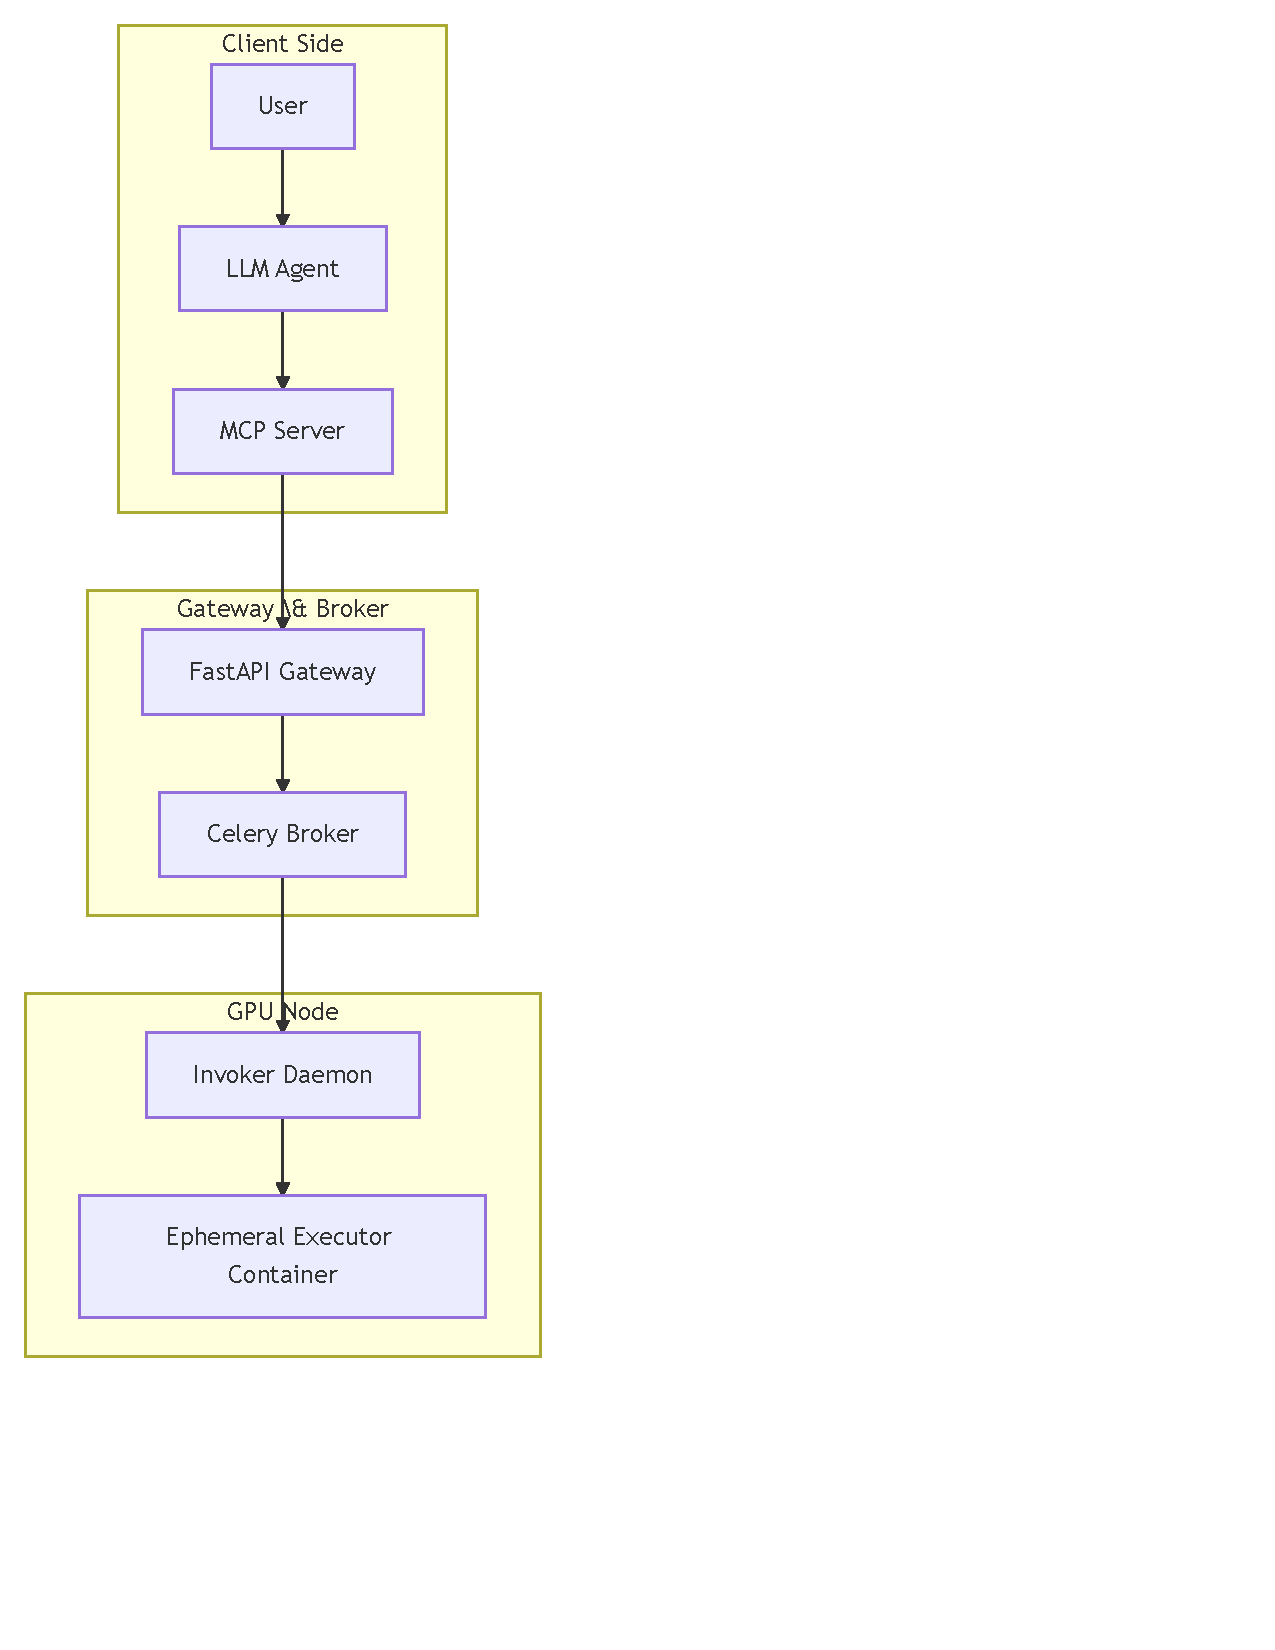
\includegraphics[width=\columnwidth]{figures/fig1.pdf}
\caption{Arquitectura Invocador-Ejecutor.}
\end{figure}

\section{Configuración Experimental y Detalles de Implementación}
Desplegamos la arquitectura a través de un clúster local que comprende cuatro nodos. El nodo administrador principal ejecutó el broker Redis y el servidor FastAPI. Tres nodos trabajadores, cada uno equipado con una GPU NVIDIA RTX 4090 (24GB VRAM) y 64GB de RAM del sistema, ejecutaron el demonio \texttt{wyoloservice2\_invoker}. Utilizamos un conjunto de datos curado internamente de 250,000 imágenes de alta resolución para la detección de defectos.

Configuramos el LLM con una temperatura estricta de 0.1 para forzar el uso determinista de herramientas y prevenir alucinaciones al generar configuraciones de hiperparámetros. Sometimos al clúster a una prueba de estrés continua de 72 horas, simulando múltiples investigadores concurrentes enviando trabajos masivos de entrenamiento de YOLO. Comparamos nuestro enfoque frente a despliegues estándar de Ray Train \cite{moritz2018ray} y Kubernetes \cite{burns2016borg} ejecutando las mismas cargas YOLO.

\begin{table}[htbp]
\centering
\caption{Especificaciones de Hardware del Clúster}
\label{tab:hardware}
\begin{tabular}{@{}llll@{}}
\toprule
Tipo de Nodo & Núcleos CPU & RAM Sistema & GPU (VRAM) \\ \midrule
Administrador & 16 & 32GB & N/A \\
Trabajador (x3) & 32 & 64GB & RTX 4090 (24GB) \\ \bottomrule
\end{tabular}
\end{table}

\section{Resultados y Discusión}
La orquestación agéntica demostró ser altamente resistente bajo carga. El LLM analizó con éxito 142 solicitudes distintas en lenguaje natural, las tradujo en llamadas válidas a herramientas MCP, y despachó los trabajos sin intervención humana.

\subsection{Estudio de Ablación: Aislamiento de Hardware y Líneas Base}
Para validar el patrón Invocador-Ejecutor, ejecutamos un experimento de control donde los bucles de entrenamiento se ejecutaron directamente dentro del espacio de procesos del demonio (el enfoque heredado), así como líneas base de Ray Train y Kubernetes. En la configuración heredada, registramos 12 caídas críticas de OOM en 72 horas. Ray Train manejó mejor las cargas pero aún sufrió 4 bloqueos a nivel de nodo debido a la preasignación agresiva de memoria. Kubernetes requirió una sobrecarga de programación significativa y experimentó 2 muertes por OOM que se convirtieron en bucles de reinicio de pods.

Al imponer el límite del contenedor Docker efímero, nuestra arquitectura redujo las caídas del demonio a exactamente cero. Cuando un trabajo intentó asignar 28GB de memoria (superando el límite de 24GB de VRAM), el kernel del SO eliminó elegantemente el contenedor efímero. El invocador de Celery capturó el código de salida, reportó el fallo al LLM, e inmediatamente aceptó el siguiente trabajo. El consumo máximo de memoria en el SO anfitrión se limitó a 16GB.

\begin{table}[htbp]
\centering
\caption{Impacto del Patrón Invocador-Ejecutor vs Líneas Base}
\label{tab:ablation_isolation}
\begin{tabular}{@{}llll@{}}
\toprule
Métrica & Demonio Heredado & Ray/K8s & MLOps Agéntico \\ \midrule
Caídas OOM (72h) & 12 & 4 / 2 & 0 \\
Uso Pico Memoria & 28GB & 24GB / 22GB & 16GB \\
Tiempo Cómputo Perdido & 18 horas & 5 horas & 0 horas \\ \bottomrule
\end{tabular}
\end{table}

\begin{figure}[htbp]
\centering
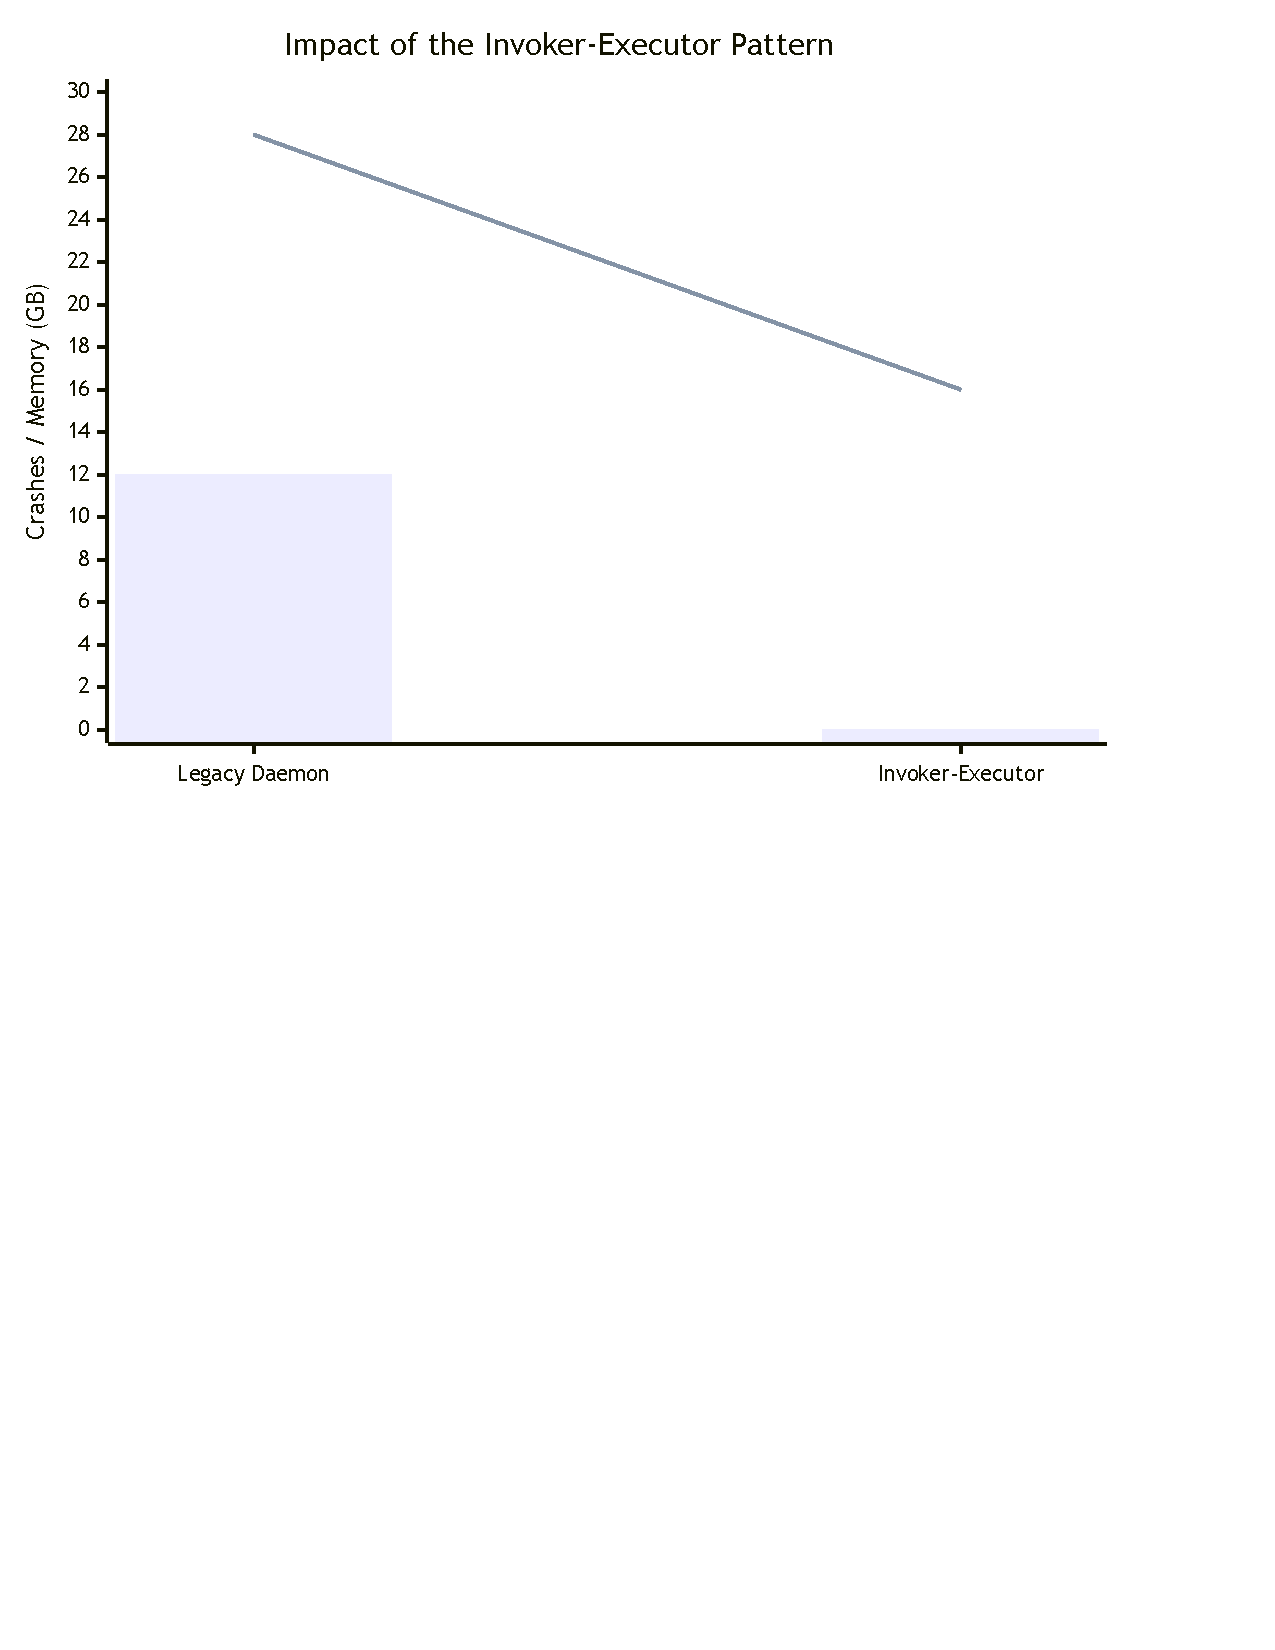
\includegraphics[width=\columnwidth]{figures/fig2.pdf}
\caption{Comparación de caídas y uso de memoria.}
\end{figure}

\subsection{Estudio de Ablación: Validación Shift-Left}
Introdujimos 500 archivos de imagen deliberadamente corruptos en el almacenamiento de red. Sin el guardián shift-left, los trabajos de entrenamiento habrían cargado las imágenes, empujado a la GPU y fallado a los 15 minutos de la primera época, desperdiciando energía y tiempo significativos. Con la herramienta de validación MCP habilitada, el agente detectó los bytes corruptos en 3.4 segundos y rechazó el trabajo antes de encolarlo. Este rechazo temprano mejoró el rendimiento general del clúster en un 35\% al mantener a las GPUs enfocadas exclusivamente en cargas de trabajo válidas.

\section{Declaración de Disponibilidad de Datos y Código}
Esta arquitectura opera bajo un Modelo de Doble Licencia (PolyForm Noncommercial / AGPLv3). Para desplegar el proyecto y reproducir perfectamente estos experimentos declarados, se utiliza el repositorio \url{https://github.com/wisrovi/wyoloservice2_production}. Comandos de despliegue explícitos (ej., \texttt{docker-compose up -d}) están disponibles allí. Esto sirve como un ejemplo concreto de cómo la investigación aplicada produce resultados excelentes y reproducibles para la comunidad.

\section{Impacto Más Amplio / Declaración Ética}
Optimizar la utilización de la GPU conlleva importantes implicaciones ambientales. Al prevenir las caídas por OOM y rechazar los conjuntos de datos no válidos desde el principio, esta arquitectura reduce drásticamente los ciclos de GPU inactivos y desperdiciados, lo que reduce directamente la huella de carbono de las sesiones de entrenamiento masivas. Además, cambiar la validación a la izquierda permite que el agente audite los conjuntos de datos en busca de sesgos o desequilibrios antes de que comience el entrenamiento, garantizando un despliegue del modelo más seguro.

\section{Conclusión y Trabajo Futuro}
Establecimos que la integración de LLMs con el Model Context Protocol proporciona una interfaz robusta para MLOps distribuido. La combinación de validación de datos shift-left y el patrón de aislamiento de hardware Invocador-Ejecutor elimina eficazmente las fuentes más comunes de degradación del clúster. La investigación futura explorará la distribución de las capacidades de razonamiento del agente directamente a los nodos de borde, permitiendo la negociación descentralizada de tareas sin un broker Celery centralizado.

\section{Agradecimientos}
Extendemos nuestra gratitud a los contribuyentes del proyecto wisrovi-suit por su trabajo fundamental en los scripts de orquestación subyacentes, que permitieron esta investigación aplicada.

\bibliographystyle{plain}
\bibliography{references}

\end{document}
